\section{Implementation}

\subsection{Overview}

The GenAI Advisor was developed using a Minimum Viable Product (MVP) approach, structured around four modular components: data ingestion, strategy engine, explanation generation, and a Streamlit-based user interface. The system was designed to be fully offline, prioritising data privacy, transparency, and reproducibility. Initial efforts focused on building a thin end-to-end pipeline to demonstrate feasibility and guide future sprints.

\subsection{System Architecture}

The overall system architecture comprises:
\begin{itemize}
    \item \textbf{Frontend:} Streamlit application for user interaction
    \item \textbf{Backend:} Modular Python packages handling data ingestion, strategy evaluation, and explanation generation
    \item \textbf{LLM Inference:} Mistral 8B model run locally via Ollama
    \item \textbf{Testing and Evaluation:} Pytest-driven unit tests and backtesting utilities
\end{itemize}

A modular layout allowed for parallel development and easier testing of individual system components. All source code and evaluation assets are available at \url{https://github.com/andreasmallios/genaiadvisor}, ensuring transparency, reproducibility, and compliance with open-source principles.

\subsection{Development Process}

An MVP-first approach guided the early stages. Agile-inspired sprints were used to iteratively add functionality and refine components. Git was used for version control, with feature branches for modular additions and frequent integration testing.

\subsection{Key Modules and Features}

\subsubsection{Data Ingestion}
Equity price data is retrieved from Yahoo Finance via the \texttt{yfinance} API, using a custom function designed to streamline data access and ensure reproducibility. The function \texttt{fetch\_ticker\_data} encapsulates logic for both online retrieval and local caching. When data for a given ticker symbol already exists in the local cache (CSV\ format), it is loaded directly using \texttt{pandas.read\_csv\(\)}, with the \texttt{Date} column parsed into a datetime index to facilitate time series analysis. This not only minimises reliance on external API calls, but also enhances the determinism of backtests.

In the absence of cached data, the function instantiates a \texttt{yfinance.Ticker} object and invokes \texttt{Ticker.history()} with a default window of one year and daily frequency. Metadata fields unrelated to price analysis (e.g., \texttt{Dividends}, \texttt{Stock Splits}) are explicitly excluded to avoid downstream noise. The retrieved data frame is then persisted locally to disk, ensuring future runs use identical input data unless manually refreshed.

All data is indexed by date, with explicit naming of the index to \texttt{Date} for consistency across modules. Additionally, the local directory used for caching is dynamically resolved using Python’s \texttt{os.path} utilities, enabling portability across environments. Although not shown directly in the function, timezone consistency is enforced at the point of usage through \texttt{tz\_localize}, ensuring temporal coherence across the ingestion and backtesting pipeline.

\subsubsection{Strategy Engine}

The strategy engine was originally implemented using a simple moving average (SMA) crossover, a well-known momentum indicator. However, it was later modularised and extended into a hybrid ensemble system, integrating both traditional technical indicators and machine learning predictions. Each strategy component was abstracted into its own module with a shared interface returning a \texttt{recommendation}, \texttt{reason}, and \texttt{date}, thereby enabling flexible composition and detailed introspection.

The indicators implemented include SMA crossover, Relative Strength Index (RSI), Moving Average Convergence Divergence (MACD), Bollinger Bands, and the Stochastic Oscillator. Each module performs well-defined signal computation:
\begin{itemize}
\item \textbf{SMA crossover}: Computes short- and long-term SMAs (50-day and 200-day by default) and identifies bullish or bearish crossovers as trading signals.
\item \textbf{RSI}: Quantifies momentum and detects overbought or oversold regimes, issuing BUY signals when RSI falls below 30 and SELL when above 70.
\item \textbf{MACD}: Uses exponential moving averages to detect momentum shifts via signal-line crossovers.
\item \textbf{Bollinger Bands}: Employs a 20-day SMA and standard deviation bands to detect volatility-based breakouts.
\item \textbf{Stochastic Oscillator}: Evaluates recent closing prices relative to the high-low range over a rolling window to spot potential reversals.
\end{itemize}

Additionally, a supervised machine learning layer was incorporated using both Random Forest and Logistic Regression classifiers. These were trained on historical technical features, including SMA differentials, RSI, MACD, returns, and volume, with future returns used as labels. Predictions from both models are aggregated and translated into BUY, HOLD, or SELL signals.

All individual signals are passed to a meta-layer defined in \texttt{engine.py}, where a weighted voting mechanism combines the recommendations. Each strategy is assigned a normalised weight, and the aggregate score is computed to produce the final advisory signal. A confidence score is also generated, which allows the user to assess the strength of the consensus recommendation.

This modular and explainable architecture enhances the system’s adaptability, allowing future indicators or models to be integrated with minimal changes to the existing pipeline.

\subsubsection{ML Implementation}

The machine learning component of the GenAI Advisor transitioned from baseline \texttt{scikit-learn} classifiers to a TensorFlow-based neural network to improve predictive performance while remaining fully auditable. Initial iterations used Random Forest and Logistic Regression to establish a benchmark, leveraging engineered features such as SMA differentials, RSI, MACD, returns, and volumes. Models and scalers were persisted to the \texttt{models/} directory to ensure reproducibility.

The final implementation employs a feedforward neural network built with TensorFlow/Keras, trained on combined historical data across all supported tickers. The network comprises two hidden layers (64 and 32 units) with ReLU activations, dropout regularisation, and a softmax output for three classes (BUY, HOLD, SELL). Labels were derived from forward ten-day price movements, with class weighting applied to mitigate label imbalance. Early stopping was used to prevent overfitting, and both the trained model (\texttt{tf\_model.h5}) and scaler were cached for inference.

This classifier is invoked within the \texttt{engine.py} pipeline via the \texttt{tensorflow\_classifier\_signal} function and integrated into the weighted ensemble in \texttt{generate\_combined\_recommendation}. Here, its output complements rule-based signals (e.g., SMA, RSI, MACD) under a defined weighting scheme. This design retains transparency by exposing model-driven rationales alongside deterministic indicators, aligning predictive improvements with the project's explainability objectives.

For inference, TensorFlow was explicitly configured to run on the CPU (\texttt{CUDA\_VISIBLE\_DEVICES=-1}) to avoid contention with the Mistral LLM, which occupies the GPU for explanation generation. Early experiments revealed that concurrent GPU usage by both TensorFlow and Mistral frequently exhausted available VRAM, causing inference failures. Running TensorFlow on the CPU mitigated these conflicts while maintaining acceptable latency for individual predictions. Although training was GPU-accelerated for efficiency, this CPU-only inference design aligns with the offline-first architecture and ensures stable operation on hardware-constrained environments without compromising model availability or reproducibility during backtesting and interactive usage.

\subsubsection{Explanation Generator}

To enhance transparency and user trust, the system includes a natural language explanation generator powered by a locally hosted instance of the Mistral 8B model, served via Ollama. This design deliberately avoids reliance on proprietary cloud APIs, enabling offline inference and preserving data privacy. Communication with the model is facilitated through Python’s \texttt{subprocess} module, which programmatically invokes the model via command-line interface.

Prompts are dynamically constructed using the metadata associated with each final recommendation. The resulting prompt embeds a structured format with three components: \textit{Summary}, \textit{Reason}, and \textit{Disclaimer}. These guide the model to produce consistent, human-readable rationales tailored for non-specialist audiences. The prompt instructs the model to contextualise signals such as SMA crossover, RSI, MACD, Bollinger Bands, Stochastic Oscillator, and ML Classifier outputs. It also emphasises educational tone, British English, and a strict 300-word limit to maintain clarity and concision.

By embedding these constraints in the prompt and invoking the model locally, the system achieves explainability without introducing dependencies that compromise reproducibility or user autonomy. Errors in generation are handled gracefully, returning informative fallback messages to aid debugging.

\subsubsection{Interface}

The user interface is developed using Streamlit, a Python-based rapid application framework tailored for data-centric interfaces. Streamlit was chosen over alternatives such as Flask or Dash due to its simplicity and tight integration with Python’s data stack, enabling rapid iteration.This decision facilitated fast prototyping and interactive visualisation, crucial during iterative development and debugging. The application enables users to input stock tickers, retrieve historical market data, view system-generated BUY, HOLD, or SELL recommendations, and inspect the rationale behind each decision.

The main interface consists of two parts: a portfolio overview and a detailed ticker analysis. The portfolio table displays summarised recommendations for all tickers within the watchlist. 

\begin{figure}[ht]
    \centering
    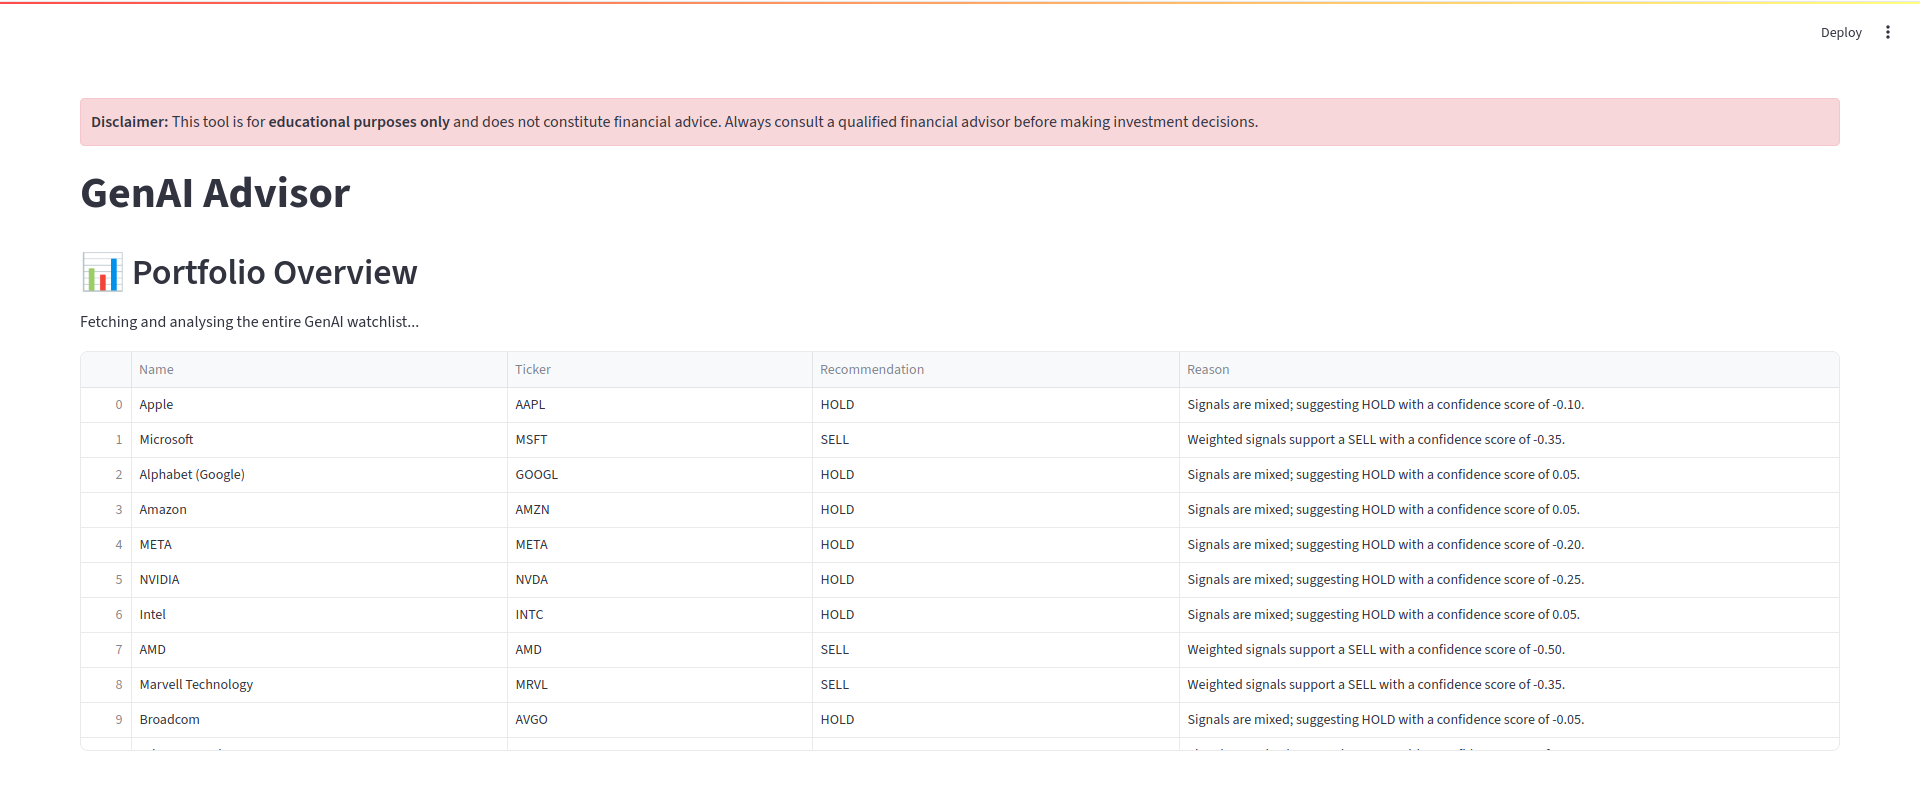
\includegraphics[width=0.9\textwidth]{assets/ui1-portfolio_overview.png}
    \caption{\small Portfolio overview, showing entire portfolio and recommendations.}
    \label{fig:ui-portfolio-overview}
\end{figure}

For deeper inspection, users may select a specific ticker, upon which the interface renders price history, a modular signal breakdown, and a natural language explanation. This layered interaction supports transparency and interpretability.

\begin{figure}[ht]
    \centering
    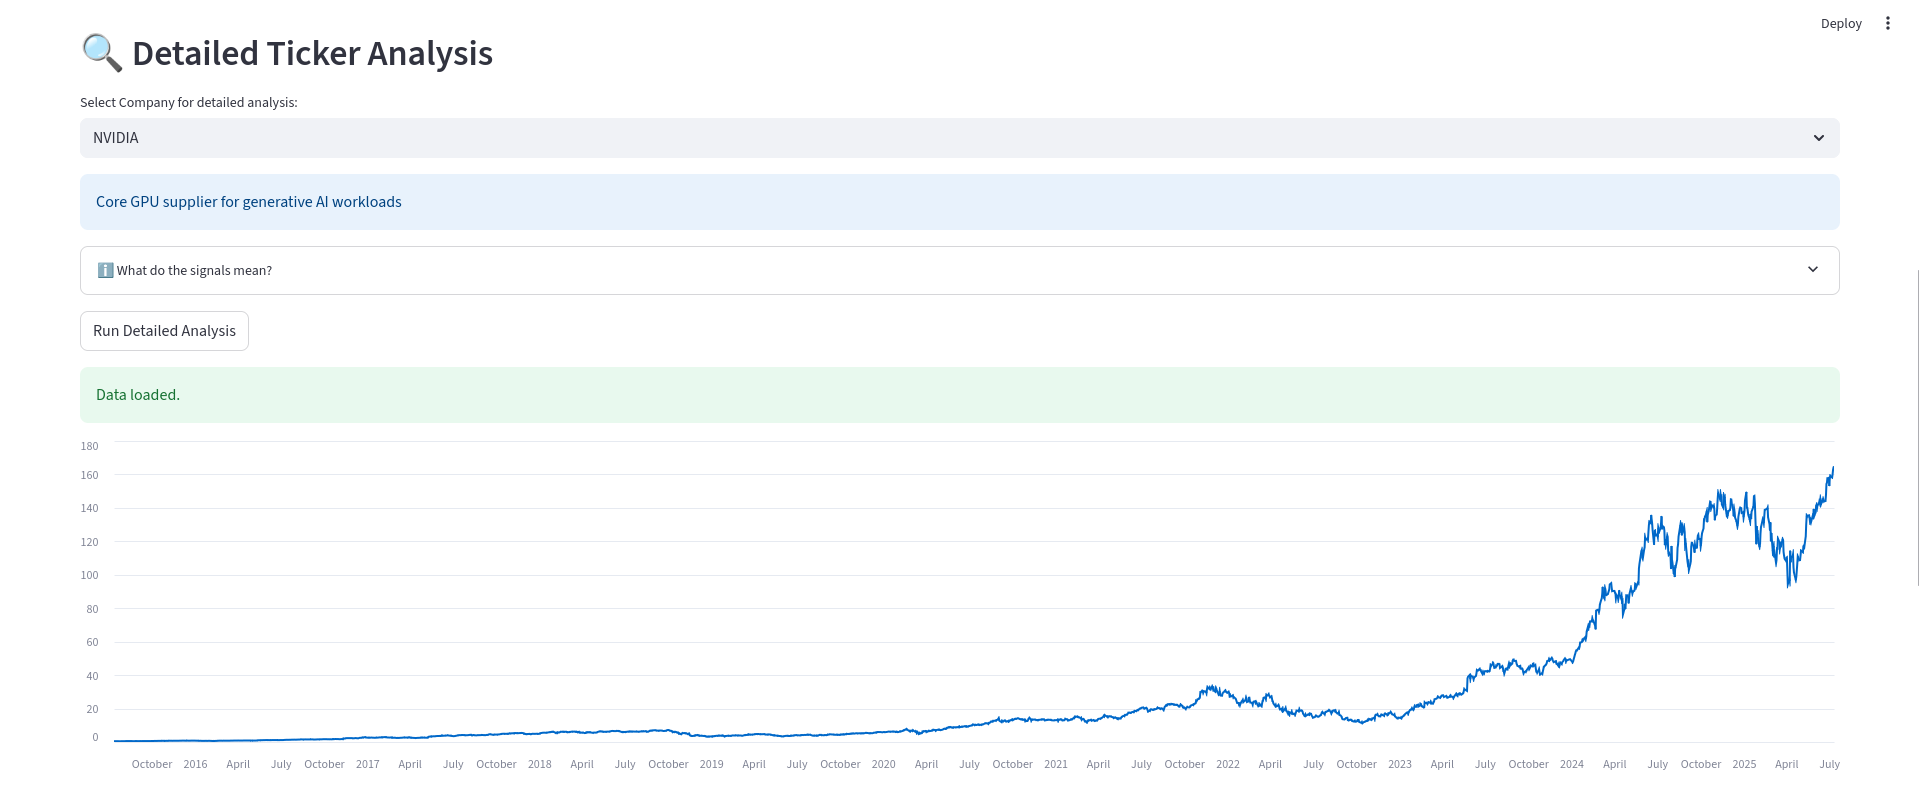
\includegraphics[width=0.9\textwidth]{assets/ui2-ticker_analysis.png}
    \caption{\small Ticker-level analysis view, showing historical price, technical signals, and explanation.}
    \label{fig:ui-ticker-analysis}
\end{figure}

Behind the scenes, the app integrates tightly with the data ingestion pipeline, database, strategy engine, and explanation generator. Recommendations and signal details are fetched dynamically and rendered as structured text. Visual aids, such as historical closing price charts, are plotted using \texttt{matplotlib} and embedded into both the interface and downloadable PDF reports. This PDF generation, facilitated by the \texttt{fpdf} library, enables offline review and archiving.

Importantly, the interface includes clear disclaimers and educational prompts, ensuring compliance with ethical guidance and reinforcing the tool’s non-advisory role. Collectively, the Streamlit-based interface serves not only as a functional front-end, but also as a pedagogical instrument that demystifies algorithmic financial decision-making for non-experts.


\subsubsection{Testing Infrastructure and Evaluation Support}

Reliability was enforced through a comprehensive \texttt{pytest} suite following Test-Driven Development (TDD) principles. Core modules—including data ingestion, technical indicators (SMA, RSI, MACD, Bollinger Bands, Stochastic Oscillator), ensemble logic, and explanation generation—were covered by dedicated tests validating type integrity, output structure, and signal consistency across edge cases.

Integration tests (\texttt{test\_engine\_call.py}) confirmed correct aggregation of weighted strategies into deterministic recommendations. The explanation generator was tested for compliance with its Summary–Reason–Disclaimer format and for robustness against subprocess errors. Pytest was executed with \texttt{PYTHONPATH=.} to resolve imports in the nested project structure.

Complementing unit testing, a batch backtesting framework replays strategy outputs against historical data, comparing predictions to forward price movements over configurable horizons (e.g., 30 days). Metrics such as hit rate, Sharpe ratio, and maximum drawdown were computed, with results logged to timestamped CSVs for notebook-based visualisation and further analysis. This dual approach—functional testing and historical simulation—ensured both software integrity and empirical grounding.

\subsubsection{Backtesting Support}

Backtesting validated the economic viability of recommendations under realistic market conditions. Using cached historical data, the system generated time-local recommendations which were benchmarked against subsequent price performance. Performance metrics included cumulative return, Sharpe ratio, maximum drawdown, and confusion matrix-derived classification accuracy.

\begin{figure}[ht]
    \centering
    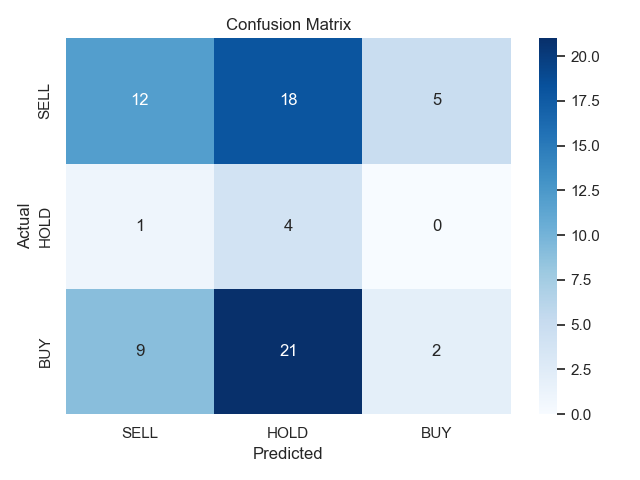
\includegraphics[width=0.65\textwidth]{assets/confusion_matrix.png}
    \caption{\small Confusion matrix of classifier predictions versus observed outcomes during evaluation.}
    \label{fig:confusion-matrix}
\end{figure}

This evaluation pipeline provided reproducible, timestamped results consistent with algorithmic trading validation best practices~\cite{bailey2014backtest}.

\subsubsection{Logging and Monitoring}

Execution logging was implemented using a lightweight CSV-based approach via \texttt{logger.py}. Each interaction, including ticker requests, generated recommendations, and explanation invocations, was appended to \texttt{logs/usage\_log.csv}. This file records timestamps, user inputs, and resulting signals, enabling both auditability and post-hoc debugging. During development, these logs were instrumental in diagnosing runtime errors and tracing data flow across modules. For example, discrepancies between model predictions and ensemble outputs were reconciled by cross-referencing log timestamps with feature generation events. This persistent logging mechanism also facilitated informal monitoring of system behaviour during backtesting and exploratory testing, thereby supporting reproducibility and transparency without requiring external monitoring frameworks.

\subsection{Environment and Dependency Management}

A Conda-based environment was used to manage dependencies and ensure reproducibility across different development machines. All required packages, including \texttt{pandas}, \texttt{yfinance}, \texttt{tensorflow}, \texttt{scikit-learn}, and \texttt{streamlit}, were defined within a single \texttt{requirements.yml} file stored at the repository root. This configuration allowed the environment to be recreated deterministically with a single command. Pinning library versions reduced the risk of incompatibilities during integration or evaluation. The approach also simplified transitions between CPU-only and GPU-enabled environments, particularly relevant for TensorFlow training versus inference runs, where GPU acceleration was explicitly disabled for deterministic CPU-bound predictions. This standardised environment setup was crucial for aligning development, testing, and report reproduction in an offline-first context.

\subsection{Code Structure and Repository Organisation}

The repository is divided into two primary components: the \texttt{code/} directory, which contains the full implementation of the GenAI Advisor, and the \texttt{report/} directory, which holds the dissertation source files.

\begin{itemize}
    \item \textbf{\texttt{code/}}: Implements the system, organised into:
    \begin{itemize}
        \item \texttt{app/} – Core application logic, including data ingestion, strategy engine, explanation generator, and supporting utilities.
        \item \texttt{data/} – Cached market data (CSV format) for reproducibility.
        \item \texttt{models/} – Trained machine learning models and scalers.
        \item \texttt{evaluation/} – Backtesting outputs and results.
        \item \texttt{logs/} – Usage logs generated during execution.
        \item \texttt{tests/} – Pytest suites aligned with application modules.
        \item \texttt{notebooks/} – Prototyping and exploratory analysis in Jupyter.
        \item \texttt{streamlit\_app/} – User interface built in Streamlit.
    \end{itemize}
    \item \textbf{\texttt{report/}}: Contains the dissertation materials:
    \begin{itemize}
        \item Chapter-wise \texttt{.tex} files and the bibliography.
        \item Figures and visualisations in \texttt{assets/}.
        \item Compiled \texttt{main.pdf} and LaTeX build artefacts.
    \end{itemize}
\end{itemize}

This structure separates implementation from documentation while maintaining cohesion within each domain, enabling systematic development and transparent academic reporting.

\subsection{Implementation Challenges}

Several technical challenges emerged during implementation, each requiring targeted debugging and design intervention.

\begin{itemize}

\item \textbf{Timezone mismatch:}\\
Historical price data retrieved via Yahoo Finance lacked explicit timezone metadata, which introduced ambiguity when slicing datasets for backtesting. This was particularly problematic when aligning cut-off dates across modules. To mitigate this, all datetime indices were explicitly localised to the \texttt{America/New\_York} timezone using the \texttt{tz\_localize} method. This normalisation ensured consistent interpretation of trading days and eliminated subtle off-by-one errors during data slicing.

\item \textbf{CSV integrity:}
Cached datasets were initially stored as CSV files to improve reproducibility and reduce API reliance. However, inconsistencies in how indices were handled during \texttt{to\_csv()} and \texttt{read\_csv()} operations led to misaligned time series and malformed DataFrames. This was addressed by explicitly setting the \texttt{index\_label} parameter during write operations and enforcing \texttt{index\_col="Date"} with \texttt{parse\_dates=True} during reads. These changes ensured referential consistency across modules and safeguarded downstream processing.

\item \textbf{Subprocess inference:}
Local model inference via the \texttt{ollama} CLI introduced challenges in handling prompt formatting, encoding, and subprocess errors. The prompt had to be programmatically composed with structured constraints while maintaining compatibility with standard input streams. Errors during model invocation (e.g., non-zero return codes) were caught and reported via Python’s \texttt{subprocess.CalledProcessError} exception handling, allowing the interface to degrade gracefully with informative fallback messages.

\item \textbf{Test discovery:}
During unit test integration, Pytest failed to resolve relative imports due to the project’s nested directory structure. This was resolved by invoking Pytest with the environment variable \texttt{PYTHONPATH=.}, thereby ensuring that all modules were discoverable relative to the project root. This solution avoided the need for path rewrites or package restructuring.

\item \textbf{Backtesting leakage:}
Initial backtest prototypes inadvertently included post-cutoff data in model inputs, leading to optimistic and invalid evaluations. This was corrected by enforcing a strict temporal cutoff: recommendations were generated using only data up to the target date, while subsequent price movements were isolated for outcome analysis. This approach ensured methodological rigour and prevented data leakage, a critical consideration in empirical evaluation.

\end{itemize}

These challenges highlight the complexity of integrating financial data pipelines, local LLM inference, and modular testing in a cohesive system. Their resolution contributed directly to the robustness and reproducibility of the final implementation.

\subsection{Summary}
This implementation unites modular financial analytics, XAI-driven explanations, and reproducible evaluation workflows in a single offline system. By adhering to robust software engineering practices, leveraging open-source tooling, and prioritising explainability, the GenAI Advisor achieves technical depth, transparency, and educational value suitable for retail investor contexts.